% ============================================================
%  Uncertainty Quantification — Thesis Defence Presentation
%  Mohd Zamin Quadri  |  TUM  |  2026
% ============================================================
\documentclass[aspectratio=169,10pt]{beamer}

\usetheme{Madrid}

% ── TUM colour palette ──────────────────────────────────────
\definecolor{tumblue}{RGB}{0,101,189}
\definecolor{tumbluedk}{RGB}{0,51,89}
\definecolor{tumlightblue}{RGB}{152,198,234}
\definecolor{tumgray}{RGB}{88,88,90}
\definecolor{tumgreen}{RGB}{0,124,48}
\definecolor{tumred}{RGB}{196,7,27}

\setbeamercolor{palette primary}{bg=tumblue,fg=white}
\setbeamercolor{palette secondary}{bg=tumbluedk,fg=white}
\setbeamercolor{palette tertiary}{bg=tumblue,fg=white}
\setbeamercolor{palette quaternary}{bg=tumbluedk,fg=white}
\setbeamercolor{structure}{fg=tumblue}
\setbeamercolor{frametitle}{bg=tumblue,fg=white}
\setbeamercolor{title}{bg=tumbluedk,fg=white}
\setbeamercolor{block title}{bg=tumblue,fg=white}
\setbeamercolor{block body}{bg=tumlightblue!20,fg=black}
\setbeamercolor{block title alerted}{bg=tumred,fg=white}
\setbeamercolor{block body alerted}{bg=tumred!10,fg=black}
\setbeamercolor{block title example}{bg=tumgreen,fg=white}
\setbeamercolor{block body example}{bg=tumgreen!10,fg=black}
\setbeamercolor{alerted text}{fg=tumred}
\setbeamercolor{item}{fg=tumblue}
\setbeamercolor{subitem}{fg=tumbluedk}

\usefonttheme{professionalfonts}
\setbeamertemplate{navigation symbols}{}
\setbeamertemplate{itemize item}{\color{tumblue}$\blacktriangleright$}
\setbeamertemplate{itemize subitem}{\color{tumbluedk}--}

% ── Packages ────────────────────────────────────────────────
\usepackage{booktabs}
\usepackage{graphicx}
\usepackage{amsmath,amssymb}
\usepackage{xcolor}
\usepackage{tikz}
\usepackage{colortbl}
\usepackage{multirow}
\usepackage{array}
\usepackage{tabularx}

% ── Convenience macros ──────────────────────────────────────
\newcommand{\emphblue}[1]{\textcolor{tumblue}{\textbf{#1}}}
\newcommand{\emphred}[1]{\textcolor{tumred}{\textbf{#1}}}
\newcommand{\emphgreen}[1]{\textcolor{tumgreen}{\textbf{#1}}}
\newcommand{\tick}{\textcolor{tumgreen}{\checkmark}}
\newcommand{\cross}{\textcolor{tumred}{$\times$}}

% ── Metadata ────────────────────────────────────────────────
\title[UQ for GNN Surrogates]{%
  Uncertainty Quantification for\\[0.2em]
  GNN Surrogates of Agent-Based Transport Models}
\author[M.\,Z.\,Quadri]{Mohd Zamin Quadri}
\institute[TUM CIT]{%
  TUM School of Computation, Information and Technology\\[0.4em]
  {\small Advisors: Dominik Fuchsgruber, M.Sc.\ \&\ Elena Natterer, M.Sc.}\\
  {\small Supervisor: Prof.\ Dr.\ Stephan G\"{u}nnemann}}
\date{Master's Thesis Defence --- 2026}

% ============================================================
\begin{document}
% ============================================================

% ── SLIDE 1: Title ──────────────────────────────────────────
\begin{frame}
  \titlepage
\end{frame}

% ── SLIDE 2: Outline ────────────────────────────────────────
\begin{frame}{Presentation Outline}
  \begin{columns}[t]
    \column{0.48\textwidth}
      \begin{block}{UQ Methods Covered}
        \begin{enumerate}
          \item[\emphblue{P1}] \textbf{Ranking Uncertainty}
            \begin{itemize}
              \item MC Dropout
              \item Selective Prediction
              \item Error Detection (AUROC)
            \end{itemize}\vspace{0.3em}
          \item[\emphblue{P2}] \textbf{Calibration}
            \begin{itemize}
              \item Why Gaussian intervals fail
              \item Temperature Scaling
              \item PIT + NLL
            \end{itemize}\vspace{0.3em}
          \item[\emphblue{P3}] \textbf{Coverage Guarantees}
            \begin{itemize}
              \item Global Conformal Prediction
              \item Adaptive Conformal Prediction
            \end{itemize}
        \end{enumerate}
      \end{block}
    \column{0.48\textwidth}
      \begin{block}{Further Experiments}
        \begin{enumerate}
          \item[\emphblue{P4}] \textbf{Ensemble Experiments}
            \begin{itemize}
              \item Exp A: Same architecture, 5 seeds
              \item Exp B: Multi-architecture ensemble
            \end{itemize}\vspace{0.3em}
          \item[\emphblue{P5}] \textbf{Negative Results}
            \begin{itemize}
              \item Trial 7: Cross-validation replication
              \item Trial 9: Heteroscedastic NLL (failure)
            \end{itemize}\vspace{0.3em}
          \item[\emphblue{P6}] \textbf{Summary \& Limitations}
        \end{enumerate}
      \end{block}
      \vspace{0.4em}
      \begin{alertblock}{Total: 13 UQ experiments}
        All on Trial 8 (best GATConv model, R$^2$=0.596)
      \end{alertblock}
  \end{columns}
\end{frame}

% ── SLIDE 3: Why UQ? ────────────────────────────────────────
\begin{frame}{Motivation: Why Do We Need Uncertainty Quantification?}
  \begin{columns}[c]
    \column{0.52\textwidth}
      \begin{block}{The Problem with Point Predictions}
        \begin{itemize}
          \item Model predicts: \emphblue{$\Delta$flow = $-3.2$ veh/hr} on road segment $i$
          \item A traffic planner acts on this number
          \item But \emphred{how reliable is this prediction?}
        \end{itemize}
      \end{block}
      \vspace{0.4em}
      \begin{alertblock}{Two road segments, same prediction value:}
        \begin{itemize}
          \item Segment A: model has seen many similar cases \tick
          \item Segment B: unusual geometry, out-of-distribution \cross
          \item \textbf{Point prediction cannot distinguish them}
        \end{itemize}
      \end{alertblock}
    \column{0.44\textwidth}
      \begin{exampleblock}{What UQ provides:}
        \vspace{0.2em}
        \centering
        \begin{tabular}{lcc}
          \toprule
          \textbf{Output} & \textbf{Value} & \textbf{Use} \\
          \midrule
          Point pred.\ $\hat{y}$ & $-3.2$ & Forecast \\
          Uncertainty $\sigma$ & $0.4$ & Trust score \\
          Interval & $[-13.2, 6.8]$ & Hard bound \\
          \bottomrule
        \end{tabular}
        \vspace{0.5em}

        \emphblue{Goal:} Make the model say not just \emph{what} it predicts, but \emph{how confident} it is.
      \end{exampleblock}
  \end{columns}
\end{frame}

% ── SLIDE 4: UQ Overview ────────────────────────────────────
\begin{frame}{UQ Framework: Three Levels of Uncertainty}
  \begin{columns}[c]
    \column{0.62\textwidth}
      \renewcommand{\arraystretch}{1.55}
      \begin{tabular}{>{\columncolor{tumlightblue!30}}p{2.4cm}
                       p{3.8cm} p{3.0cm}}
        \toprule
        \textbf{Level} & \textbf{Question answered} & \textbf{Method} \\
        \midrule
        \emphblue{1. Ranking} &
          Which predictions are least reliable? &
          MC Dropout $\sigma$ \\
        \emphblue{1. Ranking} &
          Can we improve quality by abstaining? &
          Selective Prediction \\
        \emphblue{1. Ranking} &
          Can $\sigma$ detect large errors? &
          Error Detection (AUROC) \\
        \midrule
        \emphblue{2. Calibration} &
          Are confidence scores accurate? &
          Temperature Scaling \\
        \emphblue{2. Calibration} &
          Are probability distributions correct? &
          PIT, NLL \\
        \midrule
        \emphblue{3. Guarantee} &
          Guaranteed coverage interval? &
          Global Conformal \\
        \emphblue{3. Guarantee} &
          Conditional coverage interval? &
          Adaptive Conformal \\
        \bottomrule
      \end{tabular}
    \column{0.34\textwidth}
      \begin{block}{Key Insight}
        Each level \emph{adds value}:
        \begin{itemize}
          \item Ranking $\to$ \emphblue{operational}\\(decide when to trust)
          \item Calibration $\to$ \emphblue{diagnostic}\\(is $\sigma$ meaningful?)
          \item Guarantee $\to$ \emphblue{formal}\\(provable bound)
        \end{itemize}
      \end{block}
      \vspace{0.3em}
      \begin{alertblock}{Model}
        Trial 8: PointNet + Transformer + GATConv\\
        R$^2 = 0.596$, MC $S=30$\\
        Test: 100 graphs, \textbf{3.16M} nodes
      \end{alertblock}
  \end{columns}
\end{frame}

% ============================================================
%  PART 1 — RANKING
% ============================================================
\section{Part 1: Ranking Uncertainty}

% ── SLIDE 5: MC Dropout — Method ────────────────────────────
\begin{frame}{MC Dropout: Method}
  \begin{columns}[c]
    \column{0.50\textwidth}
      \begin{block}{Standard Dropout (Training)}
        Randomly zero out neurons during training\\
        $\to$ acts as regularisation
      \end{block}
      \vspace{0.5em}
      \begin{alertblock}{MC Dropout (Inference) — Gal \& Ghahramani 2016}
        \emphred{Keep dropout active} at test time.\\
        Run $S = 30$ forward passes.
        \[
          \hat{y} = \frac{1}{S}\sum_{s=1}^{S} f_{\theta_s}(x),
          \quad
          \sigma = \sqrt{\frac{1}{S}\sum_{s=1}^{S}(f_{\theta_s}(x) - \hat{y})^2}
        \]
        $\sigma$ = \emphblue{epistemic uncertainty proxy}
      \end{alertblock}
      \vspace{0.3em}
      \begin{exampleblock}{Interpretation}
        High $\sigma$ $\to$ model disagrees with itself $\to$ \textbf{less reliable}\\
        Low $\sigma$ $\to$ model is consistent $\to$ \textbf{more reliable}
      \end{exampleblock}
    \column{0.46\textwidth}
      \centering
      \includegraphics[width=\linewidth]{slides_figs/uncertainty_hist.png}
      {\small Distribution of $\sigma$ across 3.16M test nodes.\\
      Heavy right tail = small fraction of hard cases.}
  \end{columns}
\end{frame}

% ── SLIDE 6: MC Dropout — Results ───────────────────────────
\begin{frame}{MC Dropout: Results — Is $\sigma$ Informative?}
  \begin{columns}[c]
    \column{0.46\textwidth}
      \centering
      \includegraphics[width=\linewidth]{slides_figs/binned_error_vs_uncertainty.png}
      {\small MAE increases \emph{monotonically} with uncertainty bins.\\
      This is the key diagnostic for ranking validity.}
    \column{0.50\textwidth}
      \begin{block}{Point Accuracy: Deterministic vs MC}
        \renewcommand{\arraystretch}{1.3}
        \begin{tabular}{lrrr}
          \toprule
          \textbf{Mode} & \textbf{R}$^2$ & \textbf{MAE} & \textbf{RMSE} \\
          \midrule
          Deterministic & 0.5957 & 3.96 & 7.12 \\
          MC Dropout (S=30) & 0.5857 & 3.95 & 7.21 \\
          \bottomrule
        \end{tabular}\\[0.4em]
        {\small Accuracy is comparable. MC adds $\sigma$ at marginal cost.}
      \end{block}
      \vspace{0.4em}
      \begin{alertblock}{Ranking Result}
        \textbf{Spearman $\rho$ = 0.482} between $\sigma$ and $|\text{error}|$\\[0.3em]
        Moderate-to-strong correlation.\\
        \emphblue{$\sigma$ reliably identifies harder predictions.}\\[0.3em]
        {\small Note: $\sigma$ is a ranking signal, \emph{not} a calibrated probability.}
      \end{alertblock}
  \end{columns}
\end{frame}

% ── SLIDE 7: Selective Prediction ───────────────────────────
\begin{frame}{Selective Prediction: Abstaining on Uncertain Cases}
  \begin{columns}[c]
    \column{0.46\textwidth}
      \centering
      \includegraphics[width=\linewidth]{slides_figs/risk_coverage_curve.png}
      {\small MAE drops as we reject the most uncertain predictions.\\
      X-axis = fraction of predictions retained.}
    \column{0.50\textwidth}
      \begin{block}{Method}
        Sort all 3.16M predictions by $\sigma$ (descending).\\
        Reject top-$k$\% most uncertain.\\
        Measure MAE on remaining predictions.
      \end{block}
      \vspace{0.3em}
      \begin{alertblock}{Results}
        \renewcommand{\arraystretch}{1.35}
        \begin{tabular}{rrr}
          \toprule
          \textbf{Retained} & \textbf{MAE (veh/hr)} & \textbf{Reduction} \\
          \midrule
          100\% (baseline) & 3.94 & --- \\
          90\% & 3.22 & \emphgreen{$-18.5\%$} \\
          50\% & 2.31 & \emphgreen{$-41.6\%$} \\
          25\% & 1.77 & \emphgreen{$-55.0\%$} \\
          \bottomrule
        \end{tabular}
      \end{alertblock}
      \vspace{0.3em}
      \begin{exampleblock}{Practical Value}
        A planner can choose a confidence threshold.\\
        At 90\% retention: nearly 1-in-5 improvement in accuracy\\
        \emphblue{$\sigma$ is operationally useful, not just diagnostic.}
      \end{exampleblock}
  \end{columns}
\end{frame}

% ── SLIDE 8: Error Detection ────────────────────────────────
\begin{frame}{Error Detection: Can $\sigma$ Flag Large Errors?}
  \begin{columns}[c]
    \column{0.46\textwidth}
      \centering
      \includegraphics[width=\linewidth]{slides_figs/hexbin_uncertainty_error.png}
      {\small Joint density of $\sigma$ vs.\ absolute error.\\
      High-error nodes (right) have elevated $\sigma$ (top).}
    \column{0.50\textwidth}
      \begin{block}{Binary Detection Task}
        \begin{itemize}
          \item \textbf{Positive class:} predictions in top-10\% of errors
          \item \textbf{Score:} MC Dropout $\sigma$
          \item \textbf{Question:} Does high $\sigma$ predict high error?
        \end{itemize}
      \end{block}
      \vspace{0.3em}
      \begin{alertblock}{AUROC Results}
        \renewcommand{\arraystretch}{1.3}
        \begin{tabular}{lrr}
          \toprule
          \textbf{Threshold} & \textbf{AUROC} & \textbf{AUPRC} \\
          \midrule
          Top-10\% errors & \emphblue{0.759} & 0.315 \\
          Top-20\% errors & \emphblue{0.740} & 0.455 \\
          Random baseline & 0.500 & 0.100 \\
          \bottomrule
        \end{tabular}
      \end{alertblock}
      \vspace{0.3em}
      \begin{exampleblock}{Interpretation}
        AUROC = 0.759: $\sigma$ ranks a bad prediction above a good one \textbf{75.9\% of the time}.\\
        \emphblue{52\% above random baseline} — strong discrimination.
      \end{exampleblock}
  \end{columns}
\end{frame}

% ============================================================
%  PART 2 — CALIBRATION
% ============================================================
\section{Part 2: Calibration}

% ── SLIDE 9: Why Gaussian fails ─────────────────────────────
\begin{frame}{Why Na\"{i}ve Gaussian Intervals Fail}
  \begin{columns}[c]
    \column{0.46\textwidth}
      \centering
      \includegraphics[width=\linewidth]{slides_figs/coverage_curve_k_sigma.png}
      {\small Empirical coverage vs.\ multiplier $k$.\\
      Dashed = Gaussian ideal. Actual coverage far below.}
    \column{0.50\textwidth}
      \begin{block}{Gaussian Assumption}
        Build interval: $\hat{y} \pm k\sigma$\\
        Assume $\sigma$ is a calibrated standard deviation.\\
        $k = 1.65 \to$ 90\% coverage (under Gaussian).
      \end{block}
      \vspace{0.3em}
      \begin{alertblock}{Reality: Severe Under-coverage}
        \renewcommand{\arraystretch}{1.3}
        \begin{tabular}{rrr}
          \toprule
          \textbf{Nominal} & \textbf{$k$} & \textbf{Actual coverage} \\
          \midrule
          50\%  & 0.67 & 23.3\% \\
          80\%  & 1.28 & 40.1\% \\
          90\%  & 1.65 & \emphred{48.6\%} \\
          95\%  & 1.96 & \emphred{54.8\%} \\
          \bottomrule
        \end{tabular}
      \end{alertblock}
      \vspace{0.3em}
      \begin{exampleblock}{Root Cause: Heavy-Tailed Residuals}
        Empirical $k_{95}$ = \emphblue{11.34} vs.\ Gaussian $z_{95}$ = 1.96\\
        \textbf{Ratio = 5.79$\times$} heavier tails than Gaussian\\
        $\sigma$ is a \emph{ranking signal}, not a calibrated std.\ dev.
      \end{exampleblock}
  \end{columns}
\end{frame}

% ── SLIDE 10: Temperature Scaling ───────────────────────────
\begin{frame}{Temperature Scaling: Calibrating Confidence Scores}
  \begin{columns}[c]
    \column{0.50\textwidth}
      \begin{block}{Method (Guo et al., 2017)}
        A single learnable scalar $T$ scales the logits/uncertainties:\\[0.3em]
        \[
          \sigma_{\text{cal}} = T \cdot \sigma_{\text{raw}}, \quad T > 0
        \]
        $T$ is fitted on a held-out calibration set by minimising ECE or NLL.
        \begin{itemize}
          \item $T > 1$: model was overconfident $\to$ inflate $\sigma$
          \item $T < 1$: model was underconfident $\to$ shrink $\sigma$
          \item $T = 1$: already perfectly calibrated
        \end{itemize}
      \end{block}
      \vspace{0.4em}
      \begin{alertblock}{Trial 8 Result: $T = 2.70$}
        Model was \emphred{severely overconfident}.\\
        Scaling inflated $\sigma$ by factor 2.70.
      \end{alertblock}
    \column{0.46\textwidth}
      \begin{exampleblock}{Calibration Improvement}
        \renewcommand{\arraystretch}{1.4}
        \begin{tabular}{lrrr}
          \toprule
          \textbf{Metric} & \textbf{Before} & \textbf{After} & \textbf{Change} \\
          \midrule
          ECE & 0.269 & \emphgreen{0.048} & $-82\%$ \\
          NLL & 21.65 & \emphgreen{4.75}  & $-78\%$ \\
          KS (PIT) & 0.245 & \emphgreen{0.104} & $-57\%$ \\
          \bottomrule
        \end{tabular}
      \end{exampleblock}
      \vspace{0.4em}
      \begin{block}{Residual Limitation}
        Even after scaling, \emphred{slight overconfidence persists} at high prediction magnitudes (large $|\Delta\text{flow}|$).\\[0.3em]
        $\to$ Motivates \textbf{Conformal Prediction} which gives hard guarantees without distributional assumptions.
      \end{block}
  \end{columns}
\end{frame}

% ── SLIDE 11: PIT + NLL ─────────────────────────────────────
\begin{frame}{Calibration Diagnostics: PIT and NLL}
  \begin{columns}[c]
    \column{0.50\textwidth}
      \begin{block}{PIT — Probability Integral Transform}
        If predictions $\hat{y} \sim \mathcal{N}(\hat{\mu}, \hat{\sigma}^2)$ are correct,\\
        the PIT values $u_i = \Phi\!\left(\frac{y_i - \hat{\mu}_i}{\hat{\sigma}_i}\right)$
        should be \textbf{Uniform}$[0,1]$.\\[0.4em]
        Kolmogorov-Smirnov statistic measures deviation:
        \[
          \text{KS} = \sup_u |F_{\text{empirical}}(u) - u|
        \]
        \begin{tabular}{lr}
          Raw MC: & KS = 0.245 \\
          After scaling ($T{=}2.70$): & \emphgreen{KS = 0.104} \\
          Improvement: & \emphblue{$-57\%$} \\
        \end{tabular}
      \end{block}
    \column{0.46\textwidth}
      \begin{block}{NLL — Negative Log-Likelihood}
        Measures how well the predicted distribution covers the true targets:
        \[
          \text{NLL} = \frac{1}{n}\sum_i \left[\frac{(y_i - \hat{\mu}_i)^2}{2\hat{\sigma}_i^2} + \frac{1}{2}\log\hat{\sigma}_i^2\right]
        \]
        \begin{tabular}{lr}
          Raw MC: & NLL = 21.65 \\
          After scaling: & \emphgreen{NLL = 4.75} \\
          Improvement: & \emphblue{$-78\%$} \\
        \end{tabular}
      \end{block}
      \vspace{0.3em}
      \begin{alertblock}{Summary of Calibration Evidence}
        \begin{itemize}
          \item ECE: $-82\%$ after $T=2.70$ scaling
          \item PIT/KS: $-57\%$
          \item NLL: $-78\%$
          \item All three metrics agree: \emphblue{substantial improvement}
        \end{itemize}
      \end{alertblock}
  \end{columns}
\end{frame}

% ============================================================
%  PART 3 — GUARANTEE
% ============================================================
\section{Part 3: Coverage Guarantees}

% ── SLIDE 12: Conformal Theory ──────────────────────────────
\begin{frame}{Conformal Prediction: Distribution-Free Coverage Guarantees}
  \begin{columns}[c]
    \column{0.50\textwidth}
      \begin{block}{Core Idea (Vovk et al., 2005)}
        No assumptions about residual distribution.\\
        Only requires: calibration and test data are \textbf{exchangeable}.\\[0.5em]
        \textbf{Procedure:}
        \begin{enumerate}
          \item Split test nodes into calibration (50\%) and evaluation (50\%)
          \item Compute residuals on calibration: $r_i = |y_i - \hat{y}_i|$
          \item Compute empirical quantile at level $1-\alpha$:
            \[q_\alpha = \text{Quantile}_{1-\alpha}\!\left(\{r_i\}_{i \in \mathcal{D}_\text{cal}}\right)\]
          \item Prediction interval for new point:
            \[\hat{y} \pm q_\alpha\]
        \end{enumerate}
      \end{block}
    \column{0.46\textwidth}
      \begin{alertblock}{Formal Guarantee}
        \[
          \Pr\!\left(y \in [\hat{y} - q_\alpha,\ \hat{y} + q_\alpha]\right) \geq 1 - \alpha
        \]
        This holds \emphblue{regardless of the error distribution}.\\
        No Gaussian assumption. No calibration quality assumption.
      \end{alertblock}
      \vspace{0.4em}
      \begin{block}{Important Caveat}
        This is \textbf{marginal coverage} — an average over all nodes.\\
        Per-node conditional coverage is \emph{not} guaranteed without additional methods (e.g., conformalized quantile regression).
      \end{block}
      \vspace{0.3em}
      \begin{exampleblock}{Why better than Gaussian?}
        Gaussian: assumes $\sigma$ is calibrated. It is \emphred{not}.\\
        Conformal: uses empirical residuals. \emphblue{No assumption.}
      \end{exampleblock}
  \end{columns}
\end{frame}

% ── SLIDE 13: Global Conformal Results ──────────────────────
\begin{frame}{Global Conformal Prediction: Results}
  \begin{columns}[c]
    \column{0.46\textwidth}
      \centering
      \includegraphics[width=\linewidth]{slides_figs/coverage_comparison.png}
      {\small Conformal (blue) achieves nominal coverage.\\
      Gaussian $k\sigma$ (red) severely under-covers.}
    \column{0.50\textwidth}
      \begin{alertblock}{Coverage at Nominal Levels}
        \renewcommand{\arraystretch}{1.35}
        \begin{tabular}{rrrr}
          \toprule
          \textbf{Target} & \textbf{$q$ (half-width)} & \textbf{Coverage} & \textbf{Width} \\
          \midrule
          50\%  & 1.87 & 50.35\% & 3.75 \\
          80\%  & 5.97 & 80.34\% & 11.94 \\
          \emphblue{90\%}  & \emphblue{9.99} & \emphblue{90.17\%} & 19.99 \\
          \emphblue{95\%}  & \emphblue{14.77} & \emphblue{95.09\%} & 29.54 \\
          \bottomrule
        \end{tabular}\\[0.4em]
        {\small All widths in veh/hr.}
      \end{alertblock}
      \vspace{0.3em}
      \begin{block}{Key Comparison}
        At \textbf{90\% target}:
        \begin{itemize}
          \item Gaussian $k\sigma$: actual coverage = \emphred{48.6\%}
          \item Global Conformal: actual coverage = \emphgreen{90.17\%}
          \item \emphblue{Difference: +41.6 percentage points}
        \end{itemize}
      \end{block}
      \vspace{0.2em}
      \begin{exampleblock}{Interpretation}
        For 1,000 road segments, conformal guarantees $\approx$900 have true $\Delta$flow inside the interval.
      \end{exampleblock}
  \end{columns}
\end{frame}

% ── SLIDE 14: Adaptive Conformal ────────────────────────────
\begin{frame}{Adaptive Conformal Prediction: Uncertainty-Scaled Intervals}
  \begin{columns}[c]
    \column{0.50\textwidth}
      \begin{block}{Limitation of Global Conformal}
        Fixed width $q_\alpha$ for \emph{all} predictions.\\
        Confident predictions get the same wide interval as uncertain ones.
      \end{block}
      \vspace{0.3em}
      \begin{block}{Adaptive Method}
        Scale the interval by MC Dropout $\sigma$:
        \[
          r_i^{\text{scaled}} = \frac{|y_i - \hat{y}_i|}{\sigma_i + \varepsilon}
        \]
        Compute quantile $q_\alpha^{\text{adapt}}$ on scaled residuals.\\
        Final interval: $\hat{y} \pm q_\alpha^{\text{adapt}} \cdot \sigma$
        \begin{itemize}
          \item Narrow interval where $\sigma$ is small
          \item Wide interval where $\sigma$ is large
        \end{itemize}
      \end{block}
    \column{0.46\textwidth}
      \centering
      \includegraphics[width=\linewidth]{slides_figs/interval_width_comparison.png}
      {\small Adaptive intervals adapt width to local uncertainty.}

      \vspace{0.3em}
      \begin{alertblock}{Conditional Coverage Improvement}
        \renewcommand{\arraystretch}{1.3}
        \begin{tabular}{lrr}
          \toprule
          \textbf{$\sigma$ bin} & \textbf{Global} & \textbf{Adaptive} \\
          \midrule
          Low $\sigma$ & 62.9\% & \emphgreen{90.0\%} \\
          High $\sigma$ & 98.6\% & \emphgreen{96.2\%} \\
          \midrule
          \textbf{Overall} & 90.2\% & 90.1\% \\
          \bottomrule
        \end{tabular}\\[0.3em]
        {\small Adaptive narrows the conditional coverage spread\\
        from $[62.9\%, 98.6\%]$ to $[90.0\%, 96.2\%]$.}
      \end{alertblock}
  \end{columns}
\end{frame}

% ============================================================
%  PART 4 — ENSEMBLE
% ============================================================
\section{Part 4: Ensemble Experiments}

% ── SLIDE 15: Ensemble Exp A ────────────────────────────────
\begin{frame}{Ensemble Experiment A: Same Architecture, 5 Random Seeds}
  \begin{columns}[c]
    \column{0.46\textwidth}
      \centering
      \includegraphics[width=\linewidth]{slides_figs/exp_a_mc_vs_ensemble.png}
      {\small MC Dropout $\sigma$ vs.\ ensemble variance as uncertainty proxies.}
    \column{0.50\textwidth}
      \begin{block}{Setup}
        5 instances of Trial 8, each trained with a different random seed.\\
        Ensemble variance = variance across 5 model predictions.\\
        Compare to MC Dropout $\sigma$ from single model.
      \end{block}
      \vspace{0.3em}
      \begin{alertblock}{Results: Spearman $\rho$ for uncertainty ranking}
        \renewcommand{\arraystretch}{1.3}
        \begin{tabular}{lr}
          \toprule
          \textbf{Method} & \textbf{Spearman $\rho$} \\
          \midrule
          MC Dropout $\sigma$ & \emphblue{0.491} \\
          Ensemble Variance & \emphred{0.307} \\
          \bottomrule
        \end{tabular}
      \end{alertblock}
      \vspace{0.3em}
      \begin{block}{Why ensemble variance is weaker here}
        Same architecture + same training data $\to$ \textbf{correlated errors}.\\
        Models fail \emph{together} on the same hard nodes.\\
        Ensemble variance does not capture cases where all models are simultaneously wrong.\\[0.3em]
        \emphblue{MC Dropout with single model outperforms same-architecture ensemble.}
      \end{block}
  \end{columns}
\end{frame}

% ── SLIDE 16: Ensemble Exp B ────────────────────────────────
\begin{frame}{Ensemble Experiment B: Multi-Architecture Ensemble}
  \begin{columns}[c]
    \column{0.46\textwidth}
      \centering
      \includegraphics[width=\linewidth]{slides_figs/exp_b_model_comparison.png}
      {\small Individual trial R$^2$ vs.\ weighted ensemble R$^2$.}
    \column{0.50\textwidth}
      \begin{block}{Setup}
        Weighted ensemble of 5 architecturally distinct trials:\\
        T2 + T5 + T6 + T7 + T8\\
        Weights proportional to individual R$^2$.
      \end{block}
      \vspace{0.3em}
      \begin{alertblock}{Result: Ensemble Underperforms Single Best Model}
        \renewcommand{\arraystretch}{1.3}
        \begin{tabular}{lr}
          \toprule
          \textbf{Method} & \textbf{R}$^2$ \\
          \midrule
          Trial 8 alone (best) & \emphgreen{0.596} \\
          Multi-arch ensemble & \emphred{0.566} \\
          \bottomrule
        \end{tabular}\\[0.3em]
        Also: ensemble uncertainty Spearman $\rho = 0.433$ vs.\ MC Dropout $\rho = 0.491$.
      \end{alertblock}
      \vspace{0.3em}
      \begin{block}{Lesson: Why ensembles can fail}
        \begin{itemize}
          \item Weaker models \emph{dilute} the best model's signal
          \item All trained on same 1,000 scenarios $\to$ correlated predictions
          \item Ensemble diversity requires \emph{data} diversity, not just architecture diversity
        \end{itemize}
      \end{block}
  \end{columns}
\end{frame}

% ============================================================
%  PART 5 — NEGATIVE RESULTS
% ============================================================
\section{Part 5: Negative Results}

% ── SLIDE 17: Trial 7 Cross-validation ──────────────────────
\begin{frame}{Trial 7: Cross-Validation Replication}
  \begin{columns}[c]
    \column{0.50\textwidth}
      \begin{block}{Purpose}
        Trial 8 uses an 80/10/10 split with 100 test graphs.\\
        Trial 7 uses the same split but different hyperparameters.\\
        Goal: verify UQ patterns are not artefacts of Trial 8's specific test set.
      \end{block}
      \vspace{0.4em}
      \begin{block}{Trial 7 Setup}
        \begin{itemize}
          \item Architecture: GATConv (same as T8)
          \item Dropout: 0.3 (higher than T8's 0.2)
          \item Test graphs: 100, LR: 0.0006
          \item R$^2$ = 0.547
        \end{itemize}
      \end{block}
    \column{0.46\textwidth}
      \begin{alertblock}{Key UQ Metrics — T7 vs T8}
        \renewcommand{\arraystretch}{1.35}
        \begin{tabular}{lrr}
          \toprule
          \textbf{Metric} & \textbf{T8} & \textbf{T7} \\
          \midrule
          Spearman $\rho$ & 0.482 & 0.446 \\
          $k_{95}$ & 11.34 & \emphred{16.15} \\
          Conformal $q_{90}$ & 9.99 & higher \\
          \bottomrule
        \end{tabular}
      \end{alertblock}
      \vspace{0.3em}
      \begin{block}{Interpretation}
        \begin{itemize}
          \item Pattern \emphblue{replicated}: MC Dropout still informative ($\rho = 0.446$)
          \item $k_{95} = 16.15$ vs T8's $11.34$: \emphred{higher dropout = more uncertainty spread}
          \item Gaussian intervals even more miscalibrated
          \item Confirms findings are model-independent
        \end{itemize}
      \end{block}
  \end{columns}
\end{frame}

% ── SLIDE 18: Trial 9 — Heteroscedastic Failure ─────────────
\begin{frame}{Trial 9: Heteroscedastic NLL — A Negative Result}
  \begin{columns}[c]
    \column{0.50\textwidth}
      \begin{block}{Motivation}
        Instead of post-hoc UQ (MC Dropout), train the model to output both mean \emph{and} variance directly.\\[0.3em]
        Final layer: \texttt{GATConv(64 $\to$ 2)} outputs $[\hat{\mu},\ \log\hat{\sigma}^2]$\\[0.3em]
        Loss (Kendall \& Gal, 2017):
        \[
          \mathcal{L} = \frac{1}{n}\sum_i \left[\frac{(y_i - \hat{\mu}_i)^2}{2\hat{\sigma}_i^2} + \frac{1}{2}\log\hat{\sigma}_i^2\right]
        \]
      \end{block}
      \vspace{0.3em}
      \begin{alertblock}{Result: R$^2$ = \emphred{0.02} — Near-Total Failure}
        The model learned to predict, but made completely unreliable predictions.
      \end{alertblock}
    \column{0.46\textwidth}
      \begin{alertblock}{Root Cause: Variance Inflation (Seitzer et al., 2022)}
        The NLL loss has a shortcut:\\[0.3em]
        If $\hat{\sigma}^2 \to \infty$, the first term $\to 0$ regardless of $\hat{\mu}$.\\[0.3em]
        The model learned to \emphred{inflate $\hat{\sigma}^2$} to minimise loss \emph{without} improving $\hat{\mu}$.
      \end{alertblock}
      \vspace{0.4em}
      \begin{exampleblock}{Lesson \& Fix}
        \begin{itemize}
          \item Standard heteroscedastic NLL is \emphred{insufficient} for this task
          \item Fix requires: variance head constraints, evidential deep learning (Amini et al., 2020), or decoupled mean/variance training
          \item \emphblue{Post-hoc UQ (MC Dropout + Conformal)} is more robust
        \end{itemize}
      \end{exampleblock}
  \end{columns}
\end{frame}

% ============================================================
%  SUMMARY
% ============================================================
\section{Summary}

% ── SLIDE 19: All 13 Methods Table ──────────────────────────
\begin{frame}{All UQ Experiments: Complete Summary}
  \centering
  \renewcommand{\arraystretch}{1.25}
  \footnotesize
  \begin{tabular}{llll}
    \toprule
    \textbf{\#} & \textbf{Method} & \textbf{Key Result} & \textbf{Verdict} \\
    \midrule
    1 & MC Dropout ($S=30$) & Spearman $\rho = 0.482$ & \emphgreen{\tick\ Useful ranking} \\
    2 & Gaussian $k\sigma$ intervals & 90\% nominal $\to$ 48.6\% actual & \emphred{\cross\ Miscalibrated} \\
    3 & Temperature Scaling ($T=2.70$) & ECE $-82\%$, NLL $-78\%$ & \emphgreen{\tick\ Calibrates $\sigma$} \\
    4 & PIT Diagnostic & KS $0.245 \to 0.104$ ($-57\%$) & \emphgreen{\tick\ Confirms T.S.} \\
    5 & NLL Diagnostic & $21.65 \to 4.75$ & \emphgreen{\tick\ Confirms T.S.} \\
    6 & Global Conformal & 90.02\% @ 90\% target & \emphgreen{\tick\ Guaranteed} \\
    7 & Adaptive Conformal & Conditional $[90\%, 96.2\%]$ & \emphgreen{\tick\ Better conditional} \\
    8 & Selective Prediction & $-41.6\%$ MAE @ 50\% retain & \emphgreen{\tick\ Actionable} \\
    9 & Error Detection (AUROC) & AUROC $= 0.759$ & \emphgreen{\tick\ Detects errors} \\
    \midrule
    10 & Ensemble Exp A (5 seeds) & $\rho = 0.307 <$ MC's $0.491$ & \emphred{\cross\ Correlated models} \\
    11 & Ensemble Exp B (multi-arch) & R$^2 = 0.566 <$ T8's $0.596$ & \emphred{\cross\ Diluted by weak} \\
    \midrule
    12 & Trial 7 Replication & $\rho = 0.446$, pattern holds & \emphgreen{\tick\ Cross-validated} \\
    13 & Trial 9 Heteroscedastic & R$^2 = 0.02$ & \emphred{\cross\ Variance inflation} \\
    \bottomrule
  \end{tabular}
\end{frame}

% ── SLIDE 20: 3-Level Hierarchy Recap ───────────────────────
\begin{frame}{Three-Level UQ Hierarchy: Final Picture}
  \begin{columns}[c]
    \column{0.34\textwidth}
      \begin{block}{\emphblue{Level 1: Ranking}}
        \textit{``Which predictions to trust less?''}\\[0.5em]
        MC Dropout: $\rho = 0.482$\\
        AUROC: 0.759\\
        Selective: $-41.6\%$ MAE at 50\%\\[0.5em]
        \textbf{Use:} Flag unreliable roads before deploying model output
      \end{block}
    \column{0.32\textwidth}
      \begin{block}{\emphblue{Level 2: Calibration}}
        \textit{``Are confidence scores accurate?''}\\[0.5em]
        Temp.\ Scaling $T = 2.70$\\
        ECE: $-82\%$\\
        NLL: $-78\%$, PIT KS: $-57\%$\\[0.5em]
        \textbf{Use:} Meaningful probability statements on individual predictions
      \end{block}
    \column{0.30\textwidth}
      \begin{block}{\emphblue{Level 3: Guarantee}}
        \textit{``Hard provable bounds?''}\\[0.5em]
        Global conformal:\\
        \emphblue{90.02\%} at 90\%\\
        \emphblue{95.09\%} at 95\%\\
        Adaptive: conditional $[90\%, 96.2\%]$\\[0.5em]
        \textbf{Use:} Worst-case planning for high-stakes decisions
      \end{block}
  \end{columns}
  \vspace{0.6em}
  \centering
  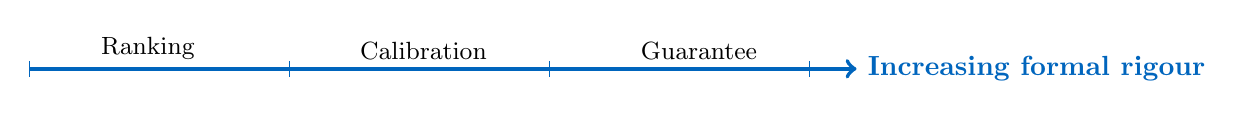
\begin{tikzpicture}
    \draw[->, line width=1.5pt, tumblue] (0,0) -- (10.5,0)
      node[right, tumblue, font=\bfseries] {Increasing formal rigour};
    \node[above, font=\small] at (1.5,0) {Ranking};
    \node[above, font=\small] at (5.0,0) {Calibration};
    \node[above, font=\small] at (8.5,0) {Guarantee};
    \foreach \x in {0,3.3,6.6,9.9} \draw[tumblue] (\x,0.1) -- (\x,-0.1);
  \end{tikzpicture}
\end{frame}

% ── SLIDE 21: Limitations ───────────────────────────────────
\begin{frame}{Limitations}
  \begin{columns}[t]
    \column{0.48\textwidth}
      \begin{alertblock}{UQ-Specific Limitations}
        \begin{itemize}
          \item \textbf{Marginal vs.\ conditional coverage:}\\
            Conformal guarantees hold on \emph{average} over all nodes — not per individual node
          \item \textbf{Calibration uses test split:}\\
            No held-out validation set was saved. Test pool was split 50/50 for conformal calibration. Standard practice but worth noting.
          \item \textbf{MC Dropout $\sigma$ is epistemic only:}\\
            Does not capture aleatoric (data) uncertainty
          \item \textbf{Heavy computational cost:}\\
            MC Dropout ($S=30$) took $\sim$228 min vs.\ deterministic $\sim$3.4 min ($67\times$ overhead)
        \end{itemize}
      \end{alertblock}
    \column{0.48\textwidth}
      \begin{alertblock}{Model \& Data Limitations}
        \begin{itemize}
          \item \textbf{Data scarcity:}\\
            1,000 of 10,000 available MATSim scenarios (10\% subset)\\
            Best GATConv model: R$^2 = 0.596$ vs.\ Elena's R$^2 = 0.78$ at 10,000 scenarios
          \item \textbf{Architecture gap:}\\
            Trial 1 (Linear head) achieves R$^2 = 0.786$ — indicates bottleneck may be in GATConv final layer
          \item \textbf{Single city:}\\
            All results on Paris network. Generalisation to other cities untested.
          \item \textbf{Heteroscedastic approach failed:}\\
            Trial 9 R$^2 = 0.02$. Native uncertainty prediction requires future work.
        \end{itemize}
      \end{alertblock}
  \end{columns}
\end{frame}

% ── SLIDE 22: Conclusion ────────────────────────────────────
\begin{frame}{Conclusion}
  \begin{columns}[c]
    \column{0.52\textwidth}
      \begin{block}{What Was Achieved}
        \begin{itemize}
          \item Applied \textbf{13 UQ experiments} on a GNN surrogate for Paris traffic
          \item Showed that MC Dropout provides a \emphblue{useful uncertainty signal} ($\rho = 0.482$, AUROC $= 0.759$)
          \item Demonstrated that \emphblue{Conformal Prediction gives hard coverage guarantees} (90.02\% at 90\% target) where Gaussian methods fail (48.6\%)
          \item Selective prediction delivers \emphblue{actionable accuracy gains} ($-41.6\%$ MAE at 50\% retention)
          \item Identified \emphred{negative results}: ensemble failure due to correlation; heteroscedastic NLL failure due to variance inflation
        \end{itemize}
      \end{block}
    \column{0.44\textwidth}
      \begin{exampleblock}{Key Numbers}
        \renewcommand{\arraystretch}{1.3}
        \begin{tabular}{lr}
          \toprule
          \textbf{Metric} & \textbf{Value} \\
          \midrule
          MC Dropout Spearman $\rho$ & 0.482 \\
          Conformal coverage @ 90\% & 90.02\% \\
          Adaptive conditional range & 90–96.2\% \\
          Selective MAE (50\% retain) & $-41.6\%$ \\
          Error detection AUROC & 0.759 \\
          ECE improvement (T.S.) & $-82\%$ \\
          Temp.\ scaling $T$ & 2.70 \\
          \bottomrule
        \end{tabular}
      \end{exampleblock}
      \vspace{0.3em}
      \begin{alertblock}{Core Message}
        \emphblue{A model that knows what it doesn't know is more useful than a more accurate model that doesn't.}
      \end{alertblock}
  \end{columns}
\end{frame}

% ============================================================
%  APPENDIX
% ============================================================
\appendix
\section{Appendix}

% ── SLIDE 23: Appendix A — k-sigma math ─────────────────────
\begin{frame}{Appendix A: Why $k_{95} = 11.34$ Instead of 1.96?}
  \begin{columns}[c]
    \column{0.50\textwidth}
      \begin{block}{Empirical $k$ Definition}
        Let $k_p$ be the value such that exactly $p$\% of test residuals satisfy:
        \[
          |y_i - \hat{y}_i| \leq k_p \cdot \sigma_i
        \]
        Under Gaussian assumptions: $k_{95} = z_{0.975} = 1.96$\\[0.3em]
        Under our heavy-tailed residuals: $k_{95} = 11.34$\\[0.3em]
        \emphred{Ratio = $11.34 / 1.96 = 5.79 \times$}
      \end{block}
      \vspace{0.4em}
      \begin{block}{What This Means}
        The residuals are much larger relative to $\sigma$ than Gaussian predicts.\\
        $\sigma$ \emph{underestimates} the spread of true errors by a factor of $\sim 6$.\\
        This is why $\hat{y} \pm 1.96\sigma$ only covers 54.8\% rather than 95\%.
      \end{block}
    \column{0.46\textwidth}
      \begin{exampleblock}{Why Heavy Tails?}
        \begin{itemize}
          \item $\sigma$ captures \emph{epistemic} uncertainty (model disagreement)
          \item True residuals also contain \emph{aleatoric} uncertainty (data noise, unseen disruptions)
          \item MC Dropout $\sigma$ has no mechanism to estimate aleatoric uncertainty
          \item Therefore $\sigma$ systematically underestimates total uncertainty
        \end{itemize}
      \end{exampleblock}
      \vspace{0.4em}
      \begin{block}{T7 Comparison}
        Trial 7 (dropout = 0.3) has $k_{95} = 16.15$\\
        Higher dropout $\to$ more stochastic $\to$ larger $\sigma$...\\
        but residuals grow even faster.\\
        \emphblue{Conformal bypasses this entirely by using empirical residuals.}
      \end{block}
  \end{columns}
\end{frame}

% ── SLIDE 24: Appendix B — Conformal proof sketch ───────────
\begin{frame}{Appendix B: Why Conformal Coverage is Guaranteed}
  \begin{columns}[c]
    \column{0.50\textwidth}
      \begin{block}{Exchangeability Assumption}
        Let $(X_1, Y_1), \ldots, (X_n, Y_n), (X_{n+1}, Y_{n+1})$ be \textbf{exchangeable} — any permutation of indices has the same joint distribution.\\[0.4em]
        This holds when calibration and test data are i.i.d.\ draws from the same distribution.
      \end{block}
      \vspace{0.4em}
      \begin{block}{Proof Sketch (Angelopoulos \& Bates, 2023)}
        The calibration residuals $r_1, \ldots, r_n$ and the test residual $r_{n+1}$ are exchangeable.\\[0.3em]
        Therefore $r_{n+1}$ is equally likely to be in any rank among $\{r_1, \ldots, r_n, r_{n+1}\}$.\\[0.3em]
        $\Pr(r_{n+1} \leq q_\alpha) \geq 1 - \alpha$ follows directly from the order statistics of exchangeable variables.
      \end{block}
    \column{0.46\textwidth}
      \begin{alertblock}{Finite-Sample Guarantee}
        With $n$ calibration points, the coverage guarantee is:
        \[
          \Pr(Y \in C(X)) \geq 1 - \alpha - \frac{1}{n+1}
        \]
        For $n = 1{,}581{,}750$ (50\% of test nodes):\\
        The correction term $\frac{1}{n+1} \approx 6 \times 10^{-7}$ is negligible.
      \end{alertblock}
      \vspace{0.4em}
      \begin{exampleblock}{No Distributional Assumptions}
        \begin{itemize}
          \item Works for any model
          \item Works for any residual distribution
          \item Works whether or not the model is well-calibrated
          \item Only fails if exchangeability is violated (covariate shift)
        \end{itemize}
      \end{exampleblock}
  \end{columns}
\end{frame}

% ── SLIDE 25: Appendix C — All trial R2 ─────────────────────
\begin{frame}{Appendix C: All Trial Results Overview}
  \centering
  \renewcommand{\arraystretch}{1.35}
  \begin{tabular}{clllrrrr}
    \toprule
    \textbf{T\#} & \textbf{Architecture} & \textbf{Key change} & \textbf{Split} & \textbf{R}$^2$ & \textbf{MAE} & \textbf{RMSE} \\
    \midrule
    1 & \emphblue{Linear} & Baseline, bs=32 & 80/15/5 & \emphblue{0.786} & 2.97 & 5.40 \\
    2 & GATConv & First GATConv, bs=16 & 80/15/5 & 0.512 & 4.33 & 8.15 \\
    3 & GATConv & Weighted loss, no dropout & 80/15/5 & 0.225 & 5.99 & 10.27 \\
    4 & GATConv & Weighted loss + dropout & 80/15/5 & 0.243 & 6.08 & 10.15 \\
    5 & GATConv & Paper config, bs=8 & 80/15/5 & 0.555 & 4.24 & 7.78 \\
    6 & GATConv & Lower LR (0.0003) & 80/15/5 & 0.522 & 4.32 & 8.06 \\
    7 & GATConv & 80/10/10, LR=0.0006 & 80/10/10 & 0.547 & 4.06 & 7.53 \\
    8 & \emphgreen{GATConv} & \emphgreen{Lower dropout (0.2)} & \emphgreen{80/10/10} & \emphgreen{0.596} & \emphgreen{3.96} & \emphgreen{7.12} \\
    9 & Heteroscedastic & NLL loss, output $[\mu, \sigma^2]$ & 80/10/10 & \emphred{0.02} & --- & --- \\
    \bottomrule
  \end{tabular}

  \vspace{0.8em}
  \begin{columns}
    \column{0.48\textwidth}
      \begin{alertblock}{Note on Trial 1}
        T1 uses \textbf{Linear} final layer — architecturally distinct from T2--T8 (GATConv).\\
        T1 R$^2=0.786$ is not directly comparable.\\
        Best \textbf{GATConv} model = T8, R$^2=0.596$.
      \end{alertblock}
    \column{0.48\textwidth}
      \begin{block}{Elena's Reference}
        Natterer et al.\ achieved R$^2 = 0.78$\\ with \textbf{10,000 scenarios} (10$\times$ more data).\\
        Our T8 uses only 1,000 scenarios (10\% subset).\\
        Data gap explains most of the R$^2$ difference.
      \end{block}
  \end{columns}
\end{frame}

% ============================================================
\end{document}
% ============================================================
